\chapter{Desenvolvimento}\label{ch:desenvolvimento}

Este capítulo apresenta o desenvolvimento do protótipo de interpretador da linguagem de programação proposta, detalhando as etapas do processo, desde o planejamento até a implementação.

O desenvolvimento do protótipo tem como objetivo, com base na seção \ref{sec:obj_geral}, provar a viabilidade inicial da implementação do \textit{design} da linguagem, além de fornecer uma base para futuras pesquisas e aprimoramentos. Assim como descrito no capítulo \ref{ch:metodologia}, o desenvolvimento foi dividido nas etapas de planejamento e implementação de modo a separar as responsabilidades do desenvolvimento.

\section{Visão Geral da Solução}

Usando como base os critérios e características do \textit{design} de linguagens de programação descritos na seção \ref{sec:design_linguagem}, o planejamento da solução foi dado pela definição de alto nível da sintaxe e semântica da linguagem, além da escolha das tecnologias a serem utilizadas na implementação do protótipo.

Já na implementação, o foco foi a construção do interpretador da linguagem proposta no planejamento, iniciando pela criação dos analisadores léxico e sintático, seguidos pela formalização da fase de interpretação. Como base para a implementação, foi principalmente utilizado o livro \textit{Crafting Interpreters} \cite{craftinginterpreters}, além de artigos sobre ECS escritos por Sander Mertens, autor da biblioteca Flecs, e documentação de bibliotecas de ECS, como Flecs \cite{flecs} e Bevy \cite{bevy}.

De modo a permitir uma visão ampla do fluxo de dados do interpretador, desde o código fonte até sua interpretação, a \autoref{fig:diagrama_atividades} apresenta o diagrama de atividades do protótipo proposto pelo trabalho.

\begin{figure}[H]
	\centering
	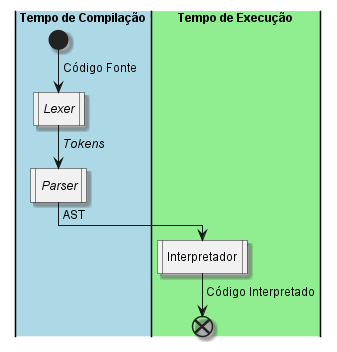
\includegraphics[width=0.25\textheight]{../diagrams/diagrama_atividades.png}
	\caption{Diagrama de atividades efetuadas pelo interpretador.}
	\fonte{Elaboração própria com PlantUML.}
	\label{fig:diagrama_atividades}
\end{figure}

Como ilustrado na \autoref{fig:diagrama_atividades}, nota-se como o fluxo de dados é igual ao de um interpretador tradicional, com apenas as fases de análise léxica, análise sintática e interpretação \cite{craftinginterpreters}. A diferença acontece na implementação por de trás dessas fases, que foram adaptadas para suportar os conceitos de ECS.

Além disso, nota-se como as atividades foram divididas nas faixas de tempo de compilação e tempo de execução. Por mais que tal distinção não terá uso prático no protótipo, ela terá uso para algumas das sugestões de pesquisas futuras, que farão uso das vantagens relacionadas ao tempo de compilação.

Entrando mais a fundo na implementação do interpretador, a \autoref{fig:diagrama_componentes} apresenta o diagrama de componentes do protótipo. Nele, nota-se o agrupamento dos três principais componentes do interpretador\footnote{A relação entre os componentes da implementação e as fases do interpretador é ilustrada na \autoref{tab:terminologia_fases}} — \textit{lexer}, \textit{parser} e interpretador — às suas respectivas fases.

Além disso, nota-se a dependência dos três componentes principais de outros componentes auxiliares, como tanto o \textit{parser} quanto o interpretador dependendo da definição de expressão. A lógica utilizada para agrupar a definição de expressão com o grupo da fase de análise sintática se deve ao fato de que é nela que expressões são criadas, enquanto o interpretador apenas as consome. A mesma lógica se aplica à todos os componentes auxiliares.

\begin{figure}[H]
	\centering
	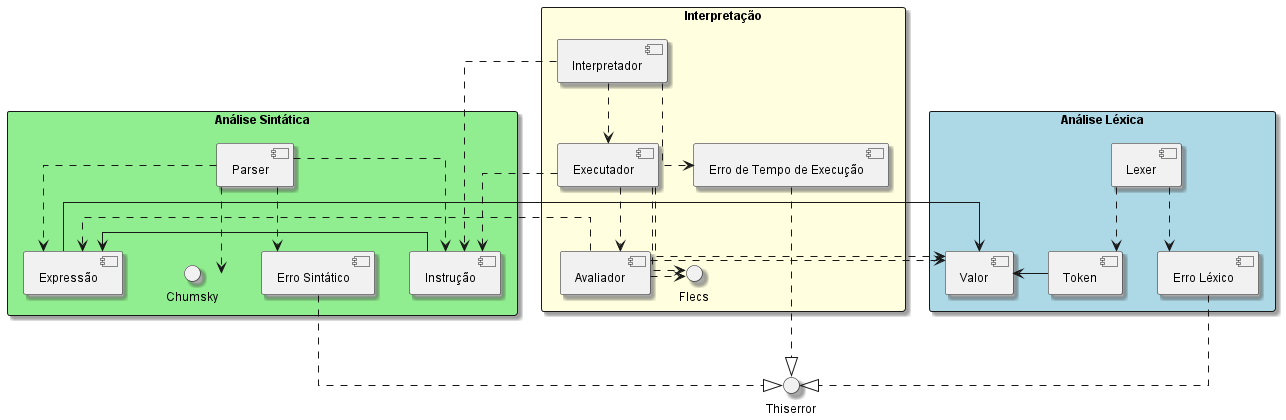
\includegraphics[width=0.65\textheight]{../diagrams/diagrama_componentes.png}
	\caption{Diagrama de componentes do interpretador.}
	\fonte{Elaboração própria com PlantUML.}
	\label{fig:diagrama_componentes}
\end{figure}

Até então, pode-se notar como foram utilizados termos como \textit{lexer} e \textit{parser} ao invés de analisador léxico e analisador sintático, respectivamente. Isso se deve ao fato de que, a partir deste ponto, esses serão os termos utilizados para se referir mais especificamente aos componentes do interpretador, enquanto os termos em português serão utilizados para se referir às fases que caracterizam estes componentes. A \autoref{tab:terminologia_fases} ilustra a diferença de uso entre os termos.

\begin{table}[h]
	\centering
	\caption{Terminologia utilizada para se referir às fases do interpretador e seus componentes.}
	{
		\begin{tabular}{ll}
			\hline
			\textbf{Fase}     & \textbf{Componente}  \\ \hline
			Análise Léxica    & \textit{Lexer}       \\
			Análise Sintática & \textit{Parser}      \\
			Interpretação     & \textit{Interpreter} \\ \hline
		\end{tabular}
	}
	\fonte{Elaboração própria com base na terminologia usada em \citeonline{craftinginterpreters}.}
	\label{tab:terminologia_fases}
\end{table}


\section{Planejamento}

Antes de iniciar o desenvolvimento do protótipo, foi realizado um planejamento com a finalidade de responder às questões de quais ferramentas utilizar, como a linguagem se pareceria, como seriam organizadas as diferentes partes do código, entre outras.

Usando como base as definições da seção \ref{sec:design_linguagem}, a linguagem proposta foi uma linguagem de programação imperativa com tipagem dinâmica, facilidando a implementação do interpretador, já que não é necessário a im
plementação de um sistema de tipos complexo.

A sintaxe foi inspirada na família de linguagens C, evidenciado pelo uso de chaves para delimitar blocos de código e instanciar componentes, ilustrado no \autoref{cod:goal_syntax}. A escolha se deve à familiaridade da sintaxe, que facilita a adoção da linguagem. Já a semântica foi inspirada na biblioteca de ECS Flecs e seu tratamento de componentes e sistemas como entidades \cite{flecs}. A escolha se deve ao potencial de flexibilidade e ortogonalidade que essa abordagem oferece, que será demonstrado pelas sugestões de pesquisas futuras.

Para a implementação do interpretador, foi escolhida a linguagem Rust. A escolha se deve principalmente pelo seu sistema de tipos, cuja utilidade será explorada na implementação do interpretador. Dentro do ecossistema Rust, a biblioteca Chumsky foi escolhida para a implementação do \textit{parser} devido a sua maturidade, facilitando a implementação em comparação com \textit{parsers} escritos do zero.

Por fim, foi criado um exemplo de código na linguagem proposta, contendo a sintaxe completa da linguagem. Ter um exemplo concreto ajudou a guiar o desenvolvimento do interpretador, servindo como um objetivo a ser alcançado. O exemplo completo pode ser visto no \autoref{cod:goal_syntax}.

\codigoRust
\lstinputlisting[
	language=Rust,
	label=cod:goal_syntax,
	caption={Exemplo de código na linguagem proposta, demonstrando de forma exaustiva sua sintaxe.}
]{../codes/goal_syntax.rs}
\vspace{-1em}
\fonte{Elaboração própria.}

O \autoref{cod:goal_syntax} consiste na definição de componentes para representar pessoas, rochas e nomes, além da criação de entidades com esses componentes e um sistema que apenas imprime o nome de pessoas, excluindo as rochas. Vale ressaltar que o código representa toda a sintaxe da linguagem, o que significa que o que não está presente não faz parte da linguagem, como reatribuição de campos e operações aritméticas. Tal falta de recursos é intencional, já que o objetivo do protótipo é explorar a viabilidade da implementação de uma linguagem com recursos de ECS em específico, e não uma linguagem tradicional.

Com a linguagem e ferramentas definidas, além do exemplo concreto de código para guiar o desenvolvimento, o planejamento foi concluído a implementação do interpretador pode ser iniciada.


\section{Implementação da Análise Léxica}

A implementação do \textit{lexer} começou com a definição de \textit{token}, que serão responsáveis por representar as palavras individuais do código-fonte e seus dados. No código, os \textit{tokens} são variantes de uma enumeração, como pode ser visto no \autoref{cod:token_enum}.

\codigoRust
\lstinputlisting[
	language=Rust,
	label=cod:token_enum,
	caption={Versão simplificada do código que define \texttt{Token} e suas variantes.},
]{../codes/token_enum.rs}
\vspace{-1em}
\fonte{Elaboração própria.}

No \autoref{cod:token_enum}, pode-se observar que as variantes \texttt{Int} e \texttt{String} carregam um valor do tipo \texttt{Value}. Esse tipo é outra enumeração, dessa vez responsável por representar os tipos de dados primitivos da linguagem, como mostrado no \autoref{cod:value_enum}.

\codigoRust
\lstinputlisting[
	language=Rust,
	label=cod:value_enum,
	caption={Versão simplificada do código que define \texttt{Value} e suas variantes.},
]{../codes/value_enum.rs}
\vspace{-1em}
\fonte{Elaboração própria.}

A escolha de representar \texttt{Token} e \texttt{Value} como enumerações (\texttt{enum}), e não como estruturas (\texttt{struct}) com um campo que indica a variante, foi motivada principalmente pelo fato de que, em Rust, \textit{pattern matching} com \texttt{match} é exaustivo, garantindo que todas as variantes sejam tratadas. Isso reduz a probabilidade de erros, como esquecer de tratar um tipo específico de \textit{token} ou valor.

Com a definição de \textit{tokens} e valores, o próximo passo foi a implementação do \textit{lexer} em si. O \textit{lexer} é responsável por ler o código-fonte caractere por caractere e agrupá-los em \textit{tokens} significativos. No caso deste trabalho, o \textit{lexer} foi implementado do zero, sem o uso de bibliotecas externas, a fim de ter mais controle na produção de erros léxicos\footnote{Em uma versão mais antiga da implementação, foi utilizada a biblioteca de análise léxica Logos. Por mais que seu uso foi capaz de reduzir dramaticamente a complexidade do código, sua funcionalidade de permitir que o usuário crie seus próprios erros léxicos ainda faltava documentação.}.

A implementação do \textit{lexer} nestre trabalho fez uso do iterador \texttt{Peekable}, incluido na biblioteca padrão de Rust, que permite olhar o próximo caractere sem consumi-lo. Podendo ver o próximo caractere a ser examinado permite descobrir padrões prematuramente para depois iniciar o consumo de um tipo de \textit{token} específico. Por exemplo, ao encontrar um caractere de aspas duplas (\texttt{"}), o \textit{lexer} sabe que deve começar a consumir um \textit{token} do tipo \texttt{String} até encontrar outra aspas duplas, simbolizando o fim da \textit{string}.

O \autoref{cod:lexer} ilustra uma versão simplificada do código que compõe o \textit{lexer}, mostrando a detecção do padrão de forma prematura para iniciar o consumo do seu respectivo \textit{token}.

\codigoRust
\lstinputlisting[
	language=Rust,
	label=cod:lexer,
	caption={Versão simplificada do código que compõe o \textit{lexer}.},
]{../codes/lexer.rs}
\vspace{-1em}
\fonte{Elaboração própria com base no \textit{lexer} implementado em Crafting Interpreters \citeonline{craftinginterpreters}.}

Com o \textit{lexer} implementado, se tornou possível transformar o código-fonte em uma sequência de \textit{tokens}, que serão utilizados na próxima etapa do processo de interpretação: a análise sintática.


\section{Implementação da Análise Sintática}

A implementação da análise sintática começou com a representação da AST pela definição das enumerações \texttt{Expr} e \texttt{Stmt}, que representam expressões e instruções, respectivamente. No código, essas enumerações são definidas como mostrado no \autoref{cod:expr_enum} e no \autoref{cod:stmt_enum}.

\codigoRust
\lstinputlisting[
	language=Rust,
	label=cod:expr_enum,
	caption={Versão simplificada do código que define \texttt{Expr} e suas variantes.},
]{../codes/expr_enum.rs}
\vspace{-1em}
\fonte{Elaboração própria.}

Sabendo que expressão é qualquer construto que retorna um valor \cite{craftinginterpreters}, a enumeração \texttt{Expr} foi definida para representar os diferentes tipos de expressões que a linguagem suporta. Junto das instruções, que são representadas pela enumeração \texttt{Stmt} ilustrada no \autoref{cod:stmt_enum}, esses dois tipos representam a AST em sua totalidade através da composição de suas variantes.

Diferente de expressões, instruções não retornam valores, e por isso, costumam ser responsáveis por alterar o estado do programa ou controlar o fluxo de execução \cite{craftinginterpreters}. A enumeração \texttt{Stmt}, ilustrada no \autoref{cod:stmt_enum}, foi definida para representar os diferentes tipos de instruções que a linguagem suporta.

\codigoRust
\lstinputlisting[
	language=Rust,
	label=cod:stmt_enum,
	caption={Versão simplificada do código que define \texttt{Stmt} e suas variantes.},
]{../codes/stmt_enum.rs}
\vspace{-1em}
\fonte{Elaboração própria.}

Vale notar a aparente contradição da variante \texttt{Stmt::Expr} no \autoref{cod:stmt_enum}. Ela existe para permitir que certas expressões sejam usadas como instruções, já que a gramática da linguagem define um programa como um conjunto de instruções. Assim, expressões como \texttt{Expr::EntityCons} podem ser tratadas como instruções quando necessário.

Com a AST representada no código, resta a implementação do \textit{parser}, que será responsável por transformar a sequência de \textit{tokens} gerada pelo \textit{lexer} em uma AST. Para isso, foi escrita a gramática formal da linguagem na notação EBNF, apresentada no \autoref{cod:grammar}.

\codigoRust
\lstinputlisting[
	language=Rust,
	label=cod:grammar,
	caption={Gramática formal da linguagem proposta na notação EBNF.},
]{../codes/grammar.ebnf}
\vspace{-1em}
\fonte{Elaboração própria.}

Note como a maioria das regras de produção tem como objetivo gerar as variantes das enumerações \texttt{Expr} e \texttt{Stmt}, salvo as regras auxiliares, como \texttt{field\_decl}, que servem para auxiliar na definição das regras principais.

Com a gramática definida, o próximo passo foi a implementação do \textit{parser} utilizando a biblioteca \textit{Chumsky}, abordada na seção \ref{sec:chumsky}. Pelo fato da biblioteca abstrair maior parte da complexidade envolvida na construção do \textit{parser}, a implementação acabou sendo um espelho direto da gramática formal definida no \autoref{cod:grammar}, como ilustrado no \autoref{cod:parser}.

\codigoRust
\lstinputlisting[
	language=Rust,
	label=cod:parser,
	caption={Versão simplificada do código que compõe o \textit{parser}.},
]{../codes/parser.rs}
\vspace{-1em}
\fonte{Elaboração própria com o uso de Chumsky \cite{chumsky}.}

Como é possível observar no \autoref{cod:parser}, as regras de produção da gramática foram traduzidas para o código de forma quase literal, salvo diferenças de sintaxe e o mapeamento das produções para as variantes das enumerações \texttt{Expr} e \texttt{Stmt}.

Vale notar o mepeamento da regra \texttt{program} para a instrução \texttt{Stmt::Block} — por mais que o programa teoricamente não seja um bloco de código, a semântica de ambos é a mesma neste trabalho, por isso, foi decidido reutilizar a variante \texttt{Stmt::Block} para representar o programa como um todo, eliminando a necessidade de criar uma nova variante apenas para esse fim.

Com a implementação do \textit{parser} concluída, o próximo passo foi interpretar a AST gerada, o que será abordado na próxima seção.


\section{Formalização da Interpretação} \label{sec:interpretacao}

Devido a restrições de tempo, a fase de interpretação não pôde ser integrada ao interpretador desenvolvido. No entanto, foram realizadas pesquisas e experimentos que podem servir como base teórica para sua implementação futura. Por isso, nesta seção será apresentado o que foi aprendido na fase de interpretação e como sua implementação pode ser abordada.

\subsection{Componentes Estáticos vs. Dinâmicos}

Ao decorrer do desenvolvimento da fase de interpretação, foi identificado que a principal dificuldade em implementar o interpretador proposto estava na representação dos componentes.

Componentes estáticos são aqueles cujo tipo é conhecido em tempo de compilação, e por isso, é necessário que o programador defina previamente todos os tipos de componentes que serão utilizados. Isso pode ser problemático em um interpretador, onde os tipos de componentes podem variar dependendo do programa que está sendo interpretado.

Em contrapartida, componentes dinâmicos permitem que os tipos sejam definidos em tempo de execução, oferecendo maior flexibilidade. Isso é especialmente útil em um interpretador, onde os tipos de componentes podem ser determinados através do código fonte que está sendo interpretado.

\subsection{Componentes Dinâmicos em Rust}

Embora componentes dinâmicos tenham sido identificados como a solução ideal, sua implementação em Rust apresentou desafios significativos. Rust é uma linguagem fortemente tipada, o que a torna menos flexível para a manipulação de tipos dinâmicos em comparação com outras linguagens.

Por outro lado, existem bibliotecas como Flecs que oferecem suporte a componentes dinâmicos em Rust. No entanto, a integração dessas bibliotecas com o interpretador exigiu um entendimento profundo de suas APIs relacionadas, que ainda não estavam completamente documentadas na época do desenvolvimento.

Para tornar concreto a diferença entre componentes estáticos e dinâmicos em Rust com Flecs, o \autoref{cod:comp_dyn_static} apresenta um exemplo simples de como criar o mesmo componente, tanto de forma estática quanto dinâmica.

\codigoRust
\lstinputlisting[
	language=Rust,
	label=cod:comp_dyn_static,
	caption={Exemplo de criação de componentes estático e dinâmico em Rust com Flecs.},
]{../codes/comp_dyn_static.rs}
\vspace{-1em}
\fonte{Elaboração própria com base em \citeonline{flecs}.}
